\documentclass[a4paper,11pt,twoside]{article}
%\documentclass[a4paper,11pt,twoside,se]{article}

\usepackage{UmUStudentReport}
\usepackage{verbatim}   % Multi-line comments using \begin{comment}
\usepackage{courier}    % Nicer fonts are used. (not necessary)
\usepackage{pslatex}    % Also nicer fonts. (not necessary)
\usepackage[pdftex]{graphicx}   % allows including pdf figures
\usepackage{listings}
\usepackage{pgf-umlcd}
\usepackage{blindtext}
\usepackage{rotating}
\usepackage{enumitem}
%\usepackage{lmodern}   % Optional fonts. (not necessary)
%\usepackage{tabularx}
%\usepackage{microtype} % Provides some typographic improvements over default settings
%\usepackage{placeins}  % For aligning images with \FloatBarrier
%\usepackage{booktabs}  % For nice-looking tables
%\usepackage{titlesec}  % More granular control of sections.

% DOCUMENT INFO
% =============
\department{Department of Computing Science}
\coursename{Development of Mobile Appliations 7.5 p}
\coursecode{5DV155}
\title{User Interface for Mobile Systems}
\author{Lorenz Gerber ({\tt{dv15lgr@cs.umu.se}} {\tt{lozger03@student.umu.se}})}
\date{2017-07-20}
%\revisiondate{2016-01-18}
\instructor{Johan Eliasson / Jonathan Westin}


% DOCUMENT SETTINGS
% =================
\bibliographystyle{plain}
%\bibliographystyle{ieee}
\pagestyle{fancy}
\raggedbottom
\setcounter{secnumdepth}{2}
\setcounter{tocdepth}{2}
%\graphicspath{{images/}}   %Path for images

\usepackage{float}
\floatstyle{ruled}
\newfloat{listing}{thp}{lop}
\floatname{listing}{Listing}



% DEFINES
% =======
%\newcommand{\mycommand}{<latex code>}

% DOCUMENT
% ========
\begin{document}
\lstset{language=C}
\maketitle
\thispagestyle{empty}
\newpage
\tableofcontents
\thispagestyle{empty}
\newpage

\clearpage
\pagenumbering{arabic}

\section{Introduction}
The aim of this assignment is to translate a desktop mail client application to
a mobile app. This includes both functional and design related aspects. The
functionality shall be described in terms of Android elements and concepts such
as activities, layouts, menues, dialogs, fragments and messages. A main aspect is
to decide and reason which functionality should be stripped from the desktop version
and eventual additional functionality needed in the mobile app.

The design shall account for usability aspects following concepts from the
course litterature \cite{clark2015} and platform guidelines \cite{materialdesign}.
The report has to include several prototype designs of which at least one shall be
made in `Android Studio' and one by hand or any design/drawing application of choice.

Further, one section of the report shall describe differences and changes in the
design when the proposed Android application would be ported to another mobile
platform of choice.

\section{The Desktop Mail Client - Apple Mail}
Here the 'Apple Mail' client was chosen as desktop application to be ported to
an Android mobile app. The version at hand was 10.3 (3273) in a macOS Sierra
Environment (10.12.5). Initially, a systematic inventory of the available
functionality in Apple Mail was conducted.

\subsection{Description of main UI of Apple Mail}
The main UI of Apple Mail is shown in figure \ref{fig:apple_main_screen}.
It consists of three columns of which only the `Mail List' and `Mail Details'
column are shown by default. The `Mail List' presents all mails of the active mailbox.
the list entry can be customised in the `Preferences', accessible through the `File'
drop down menu. The `Mail List' has by default a sort/filter bar with a drop down
menu for various list sort methods and an icon button to apply filters. The `Mail
List' scrolls vertically when not all mails of the mailbox fit on the screen.
Inspired by the Apple iOS interface, mail list items implement horizontal swipe
actions. By default, to the right for deleting and to the left for toggling
read/unread.

The `Mail Details' frame shows the detail view of one email, the one selected in
the `Mail List'. This view scrolls if needed both vertically and horizontally.
Various options regarding the visualization can be chosen in the `Preferences'
menu. By default, the header of the mail contains a number of `hyperlink' style
functionality for toggling visibility of some less often needed information but
also as shortcut for the common mail actions `Delete', `Reply', `Reply to all',
`Forward' and access to attachments.

The `Mailbox List' column can be toggled visible/invisible
by a button in the `Favorites' bar which otherwise contains text buttons for the
available mailboxes. The `Mailbox List' in combination with the `Mail List' offers
extensive `drag \& drop' functionality to put mail messages from one folder to
another.

Above the `Favorites' bar there is the `Toolbar' that contains in the default
setup nine buttons and a search field. The buttons are from left to right:
`Get new messages', `Compose new mail', `Archieve selected', `Delete selected',
`Selected to junk', `Reply', `Reply All', `Forward' and `Flag selected'. The
search field allows for text search in all or in a specific mailbox. Both
the content and the layout of the `Toolbar' is freely customizable with a number
of addtional functions/buttons not visible in the default setup.

Both the `Mail Message' and the `Folder' object on the screen provide context
sensitive menu on 'right-click'.

\begin{figure}
  \centering
    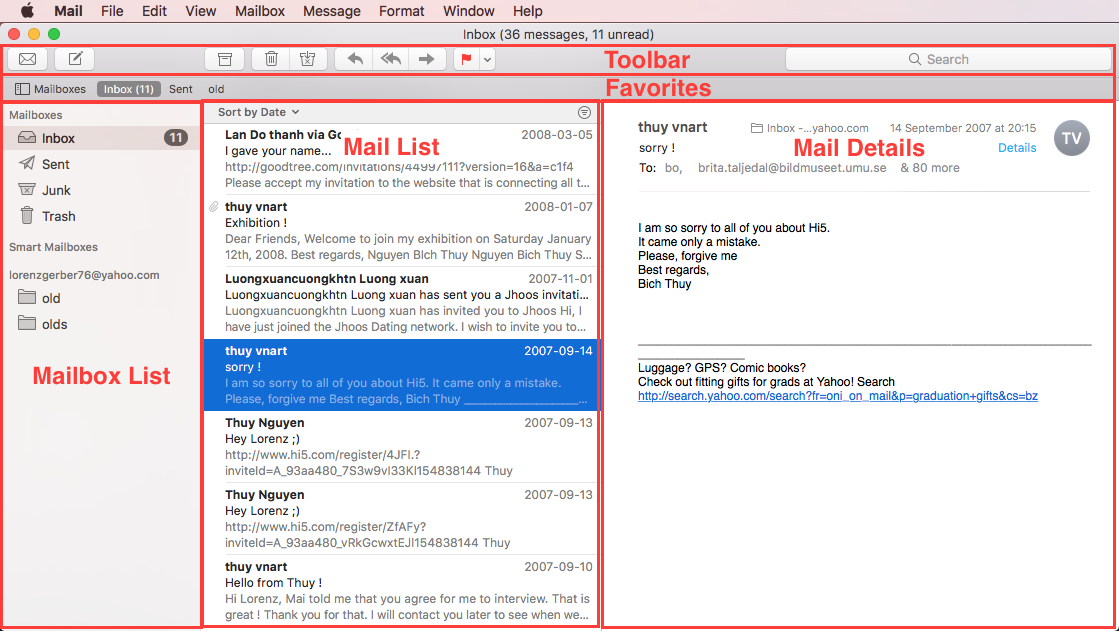
\includegraphics[width=1\textwidth]{main_screen}
    \caption{\textit{The main view of Apple Mail has three columns: `Mailbox List',
    `Mail List' and `Mail Details'. The `Mailbox List' column is however
    hidden in the standard configuration.}}
    \label{fig:apple_main_screen}
\end{figure}

\subsection{Description of Menu accessible Functionality in Apple Mail}
The `Menu Bar' contains the dropdown menus `File', `Edit', `View', `Mailbox',
`Message', `Format', `Windows' and `Help'. Most of the menu items are functionality
that is also directly accessible in the UI. The menu shows keyboard shortcuts for
much of the functionality. Menu items not found in the UI are either for
configuration and customizing the UI, or for setting up and configuring the user
data such as mailboxes accounts and smart assitant functions.

\subsection{Notifications}
Being a an application developed by `Apple' itself, `Apple Mail' is fully integrated
with the OSX notification center and offers as such a wide range of configuration to
adapt notification behaviour to the users preferences \cite{apple_notifications}. The
main elements of the notification system is a small badge that shows up in the upper
right screen corner and floats for several seconds over all other content on the
screen until it dissapears again. Apple Mail uses this notification badge when a
new a new mail message is received. All notification messages are collected and
archieved in the notification center which slides in as a drawer on the right side
of the screen when pressing the notifications icon in the main menu bar. Further,
the number of unread mails is shown in the application icon on the macOS `Dock'.

\section{Establishing the Mobile Application Profile}
The core functionality of a mail application is receiving, writing and sending
mail messages. Mail Message, Mail account and Mailbox administration is
secondary functionality. A desktop application like `Apple Mail' offers the
full package of primary and secondary functionality. More over, a wealth of
settings to tailor parts of the layout and application envelope according to the
user preferences.

Here it is assumed that the application profile of mobile
mail client users is by default more limited. A mobile application does not need
to offer the same flexibilty for customization and the profile of available
functions will be more narrow.

The most important functionality for a mobile mail client user is to have easy
access to the newest information. This includes receiving messages, getting
informed about new messages, quick access to new messages but also convenient
access methods for old messages. Writing new mail messages is of lower
importance. For quick informal messages most people use nowadays special
message/chat application that offer a more direct type of communication and
interaction with people. Further, it is not very convenient to type and layout
longer mail messages with the on-screen keyboard on mobile device compared to a
real physical keyboard. All sort of administration functionality besides setting
up multiple mail accounts is considered of lowest priority in the mobile mail
client.

Hence the following prioritized list of functionality resulted for the mobile
application.
\begin{enumerate}
  \item Receive and Present new Mail Messages
  \item Search for Mail Messages
  \item Write and Send Mail Messages
  \item Account Administration and Organization
\end{enumerate}



\section{Transforming the Desktop Applicatin to an Android App}
\subsection{The Application Structure}
While a desktop application has very little space constraints and can
compartmentalize the main screen in different sub containers, the mobile app
uses mostly one screen for one purpose. In Android Framework terms: One `Activity'
for one purpose. For reasons of modularization and
reuseability, there is often used a second layer of abstraction, the
Fragment.  The desktop app has two main containers, `Mail List' and `Mail
Details'.

\begin{sidewaysfigure}[hp!]
    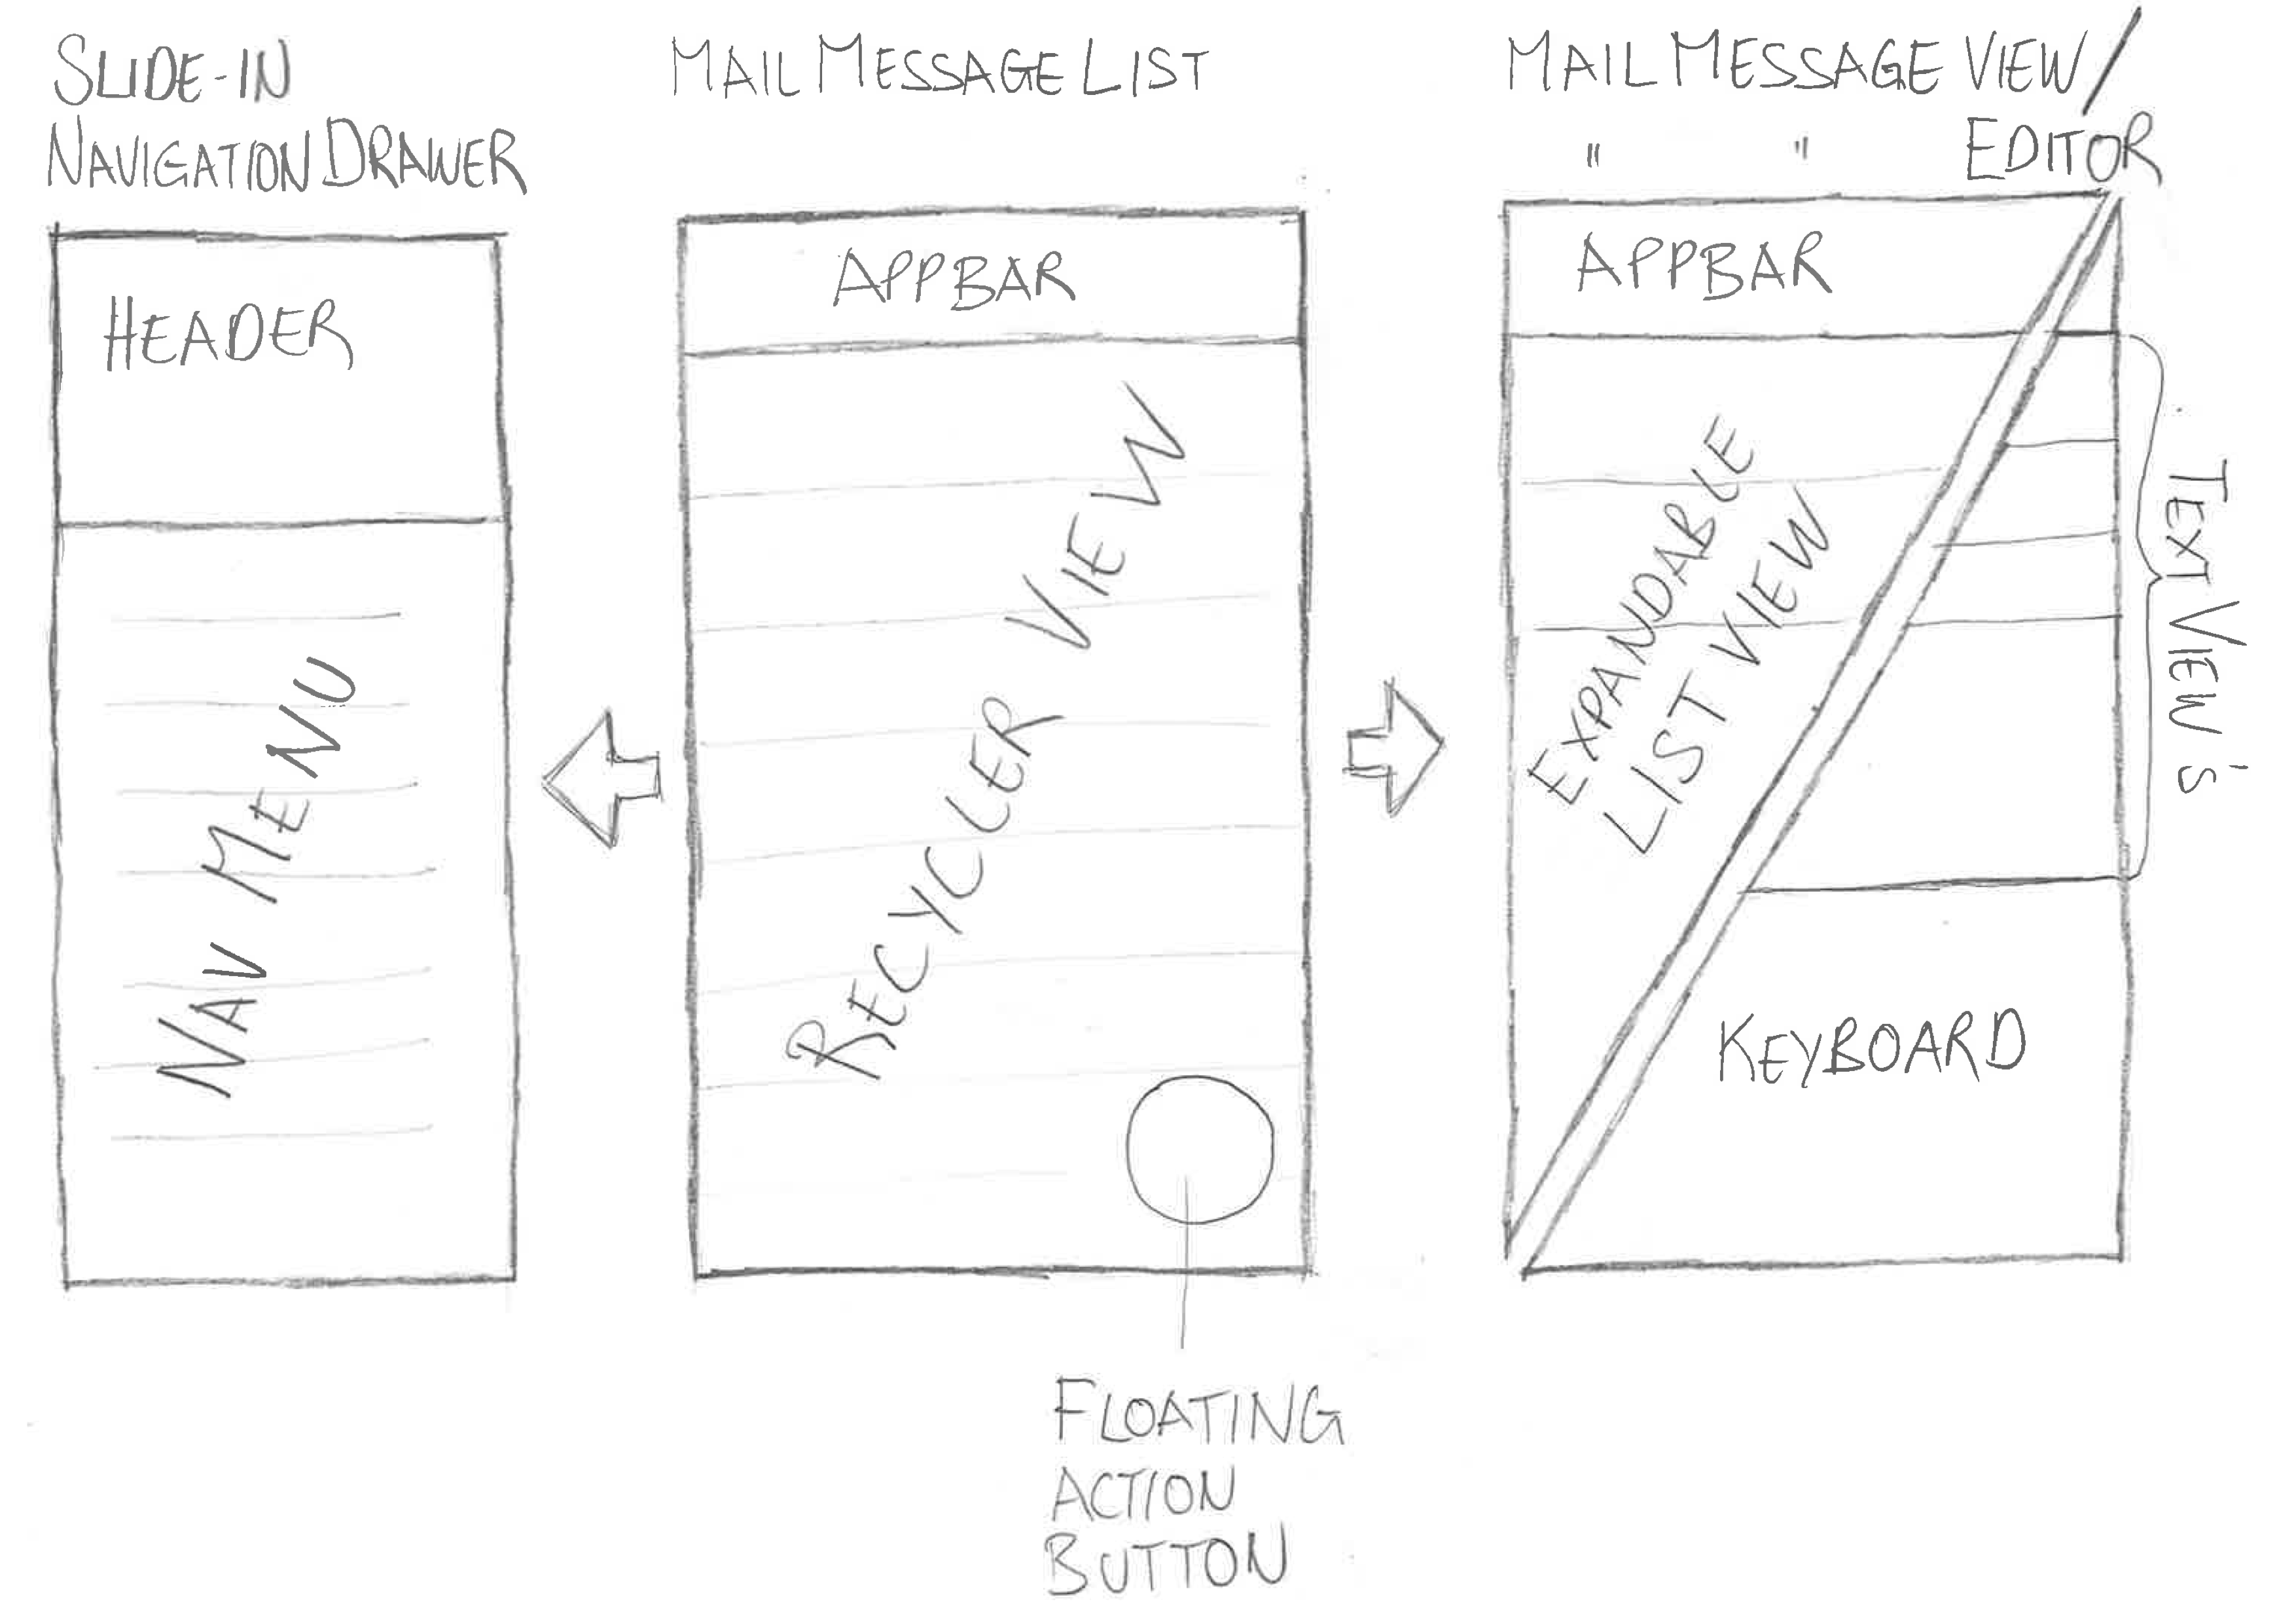
\includegraphics[width=1\textwidth]{hand_design.png}
    \caption{Design draft on the Android Mail Client.}
    \label{fig:hand_design}
\end{sidewaysfigure}

The Android app is will split the containers into separate screens or
in Android Framework terms, `Activities'. As a second layer of abstraction,
there will also be used `Fragments'. The overall layout is showcased in
figure \ref{fig:hand_design}:   The `Mail List', represented by the middle
outline, there will be one fragment in the corresponding activity. For `Mail Details',
the right-most outline in figure \ref{fig:hand_design}, there will be a `Show Mail' and
a `Edit Mail' fragment in the same `Mail Details' activity. The desktop
`Mailbox List' which is a foldable column in the desktop application is translated
into a material design `navigation drawer' (see \cite{navigation_drawer}) that
slides in from the left side, (left-most outline in figure \ref{fig:hand_design}).

For notifications, the usual Android infrastructure is used: On arrival, new messages
peek for a short period into the active screen. This notification will allow
support opening up the `Mail Detail' view.  Then unread messages are indicated
by an icon in the status bar. The notifciation is also added to the Android
`Notification Drawer' \cite{android_notifications}.

\subsection{Application Design Elements and User Experience}
While studying the Android Material Design guidelines, it was striking how well
they align with the topics in the course litterature \cite{clark2015}. Material
Design Components offer many ways of direct interaction that allow building
a fast and intuitive UI as described in Clark 2015
(\cite[chapter 3, 'Enable primary tasks directly from list view']{clark2015}).


\subsection{Detailed Layout and Design Description}
To devise more detailed design descriptions of each part in the mobile app,
setting up mock-ups in Android Studio was chosen. To obtain mockups that
include certain dynamic functionality, some mockup classes and data had to be
included. A repository with the respective android studio project can be found
here: \url{https://github.com/lorenzgerber/designmailclient.git}.

\subsubsection{Scrollable Mail Message List}
A mockup created in Android Studio of the scrollable `Mail Message List' can be
seen in figure \ref{fig:mail_message_list}. Technically, the implementation
usese a `RecyclerView' within a `CoordinatorLayout'. The former allows for
resuse and efficient caching of the the list items. The latter is used to allow
interactions between child elements. There will be a number of such interactions
described further down.

\begin{figure}[hp!]

  \centering
    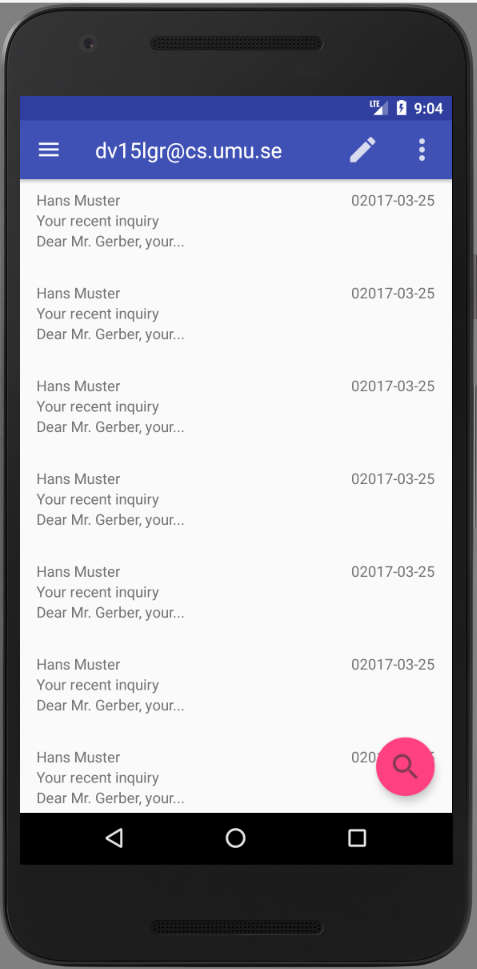
\includegraphics[width=0.5\textwidth]{mail_message_list}
    \caption{\textit{The main view of Apple Mail has three columns: `Mailbox List',
    `Mail List' and `Mail Details'. The `Mailbox List' column is however
    hidden in the standard configuration.}}
    \label{fig:mail_message_list}
\end{figure}

The list item shall according to Material Design guidelines have no more
than  three lines \cite{material_lists}. Here, the first line is used for the
Mail Message senders name and the timestamp when the message was recevied. The
second line shows the subject and the third the first text line of the message.

The primary direct interaction of this view is to scroll up and down in the
`Mail Message List' and choose a message for the `Mail Detail View' by tapping
on the list item.

The toolbar uses the Material Design component `AppBarLayout'
\cite{appbar_layout}. It hosts the menu icon on the left to swipe in the
`Navigation Drawer', a title showing the current active mail account and an
`ImageButton' icon to compose a new mail message.

The `AppBarLayour' provides functionality for advanced scrolling
techniuqes of the underlying content, for exampel `Swipe to Refresh' at
the top of the recycler list \ref{fig:mail_message_list}.
When pull down the list that is already in top end
position, the active mail account will be queried for new messages. The
implementation of this primary action (reload mailboxes) is a good example
of an intuitive UI: The user expects the newest mails to be on top of the list.
It is understood that the list can be scrolled. When the user wants to check if
the current visible message is the newest, he will automatically pull the list
down and by this activate a mailbox reload. When a new messages is downloaded
from the server, a `snackbar' message shows up to give a distinct signal to the
user that new messages are available.

Another direct interaction that implements primary funcitonality is the
horizontal swiping of list elements \cite['Leave-behinds']{material_list_controls}.
In `Apple Mail', swiping to the right will
mark the message as `unread' while swiping to the left will delete it. This seems
a rather dangerous combination for a mobile user interace. Therefore it was
decided that left and right swipe will trigger the
same function. According to Clark (\cite[chapter1, `Hold the
phone']{clark2015}), most people hold the device initially in the right hand,
but then switch frequently. According to Clark, in one hand operation, using the
thumb is predominant. It was considered  that for one hand operation with the
thumb, the natural understanding of interaction would be to swipe a list element
away from the user. But as the user frequently changes the hand that holds the
device, applying the same function for left and right swipe seems most
consistent and safe. When a message is archieved in that way, a `snackbar'
message appears at the bottom of the screen.

It was also decided to only trigger archieving of Mail Messages, no delete
action  which is in contrast to several popular mail apps. Often the choice
between archieve  or delete depends on the type of the underlying mail account:
Not all mail accounts provide archieve functionality. The app under development
will address this issue with a software based solution. This is however not
in the scope of this report.

Clark makes a point that the Android setup with three system buttons on the
screen bottom is less than optimal: Folllowing design rules, it prevents from
placing app specific functionality to there  (
\cite[Chapter 1, 'Make Way for the Operating System']{clark2015}).
And indeed Google material design only  has a
few components that could violate this rule. As fix, several components are
provided that help to circumvent this Android system design limitation. One of
them is the Floating action button (FAB) which allows to place some primary
functionality in a easily reachable area. Here the FAB was implemented for mail
message searching.

\subsubsection{Navigation Drawer}
The navigation drawer is an element within the `Mail Message List' Activity. A
Material Design Component is available to help implement typical behaviour of
the Navigation drawer, which includes the menu item at the left edge of the appbar
that will slide in the drawer from the left. The more direct way of
sliding in the drawer is to swipe inwards from the left edge of the screen: This
feels arguably like a intuitive physical interaction.

\begin{figure}[hp!]
  \label{fig:nav_drawer}
  \centering
    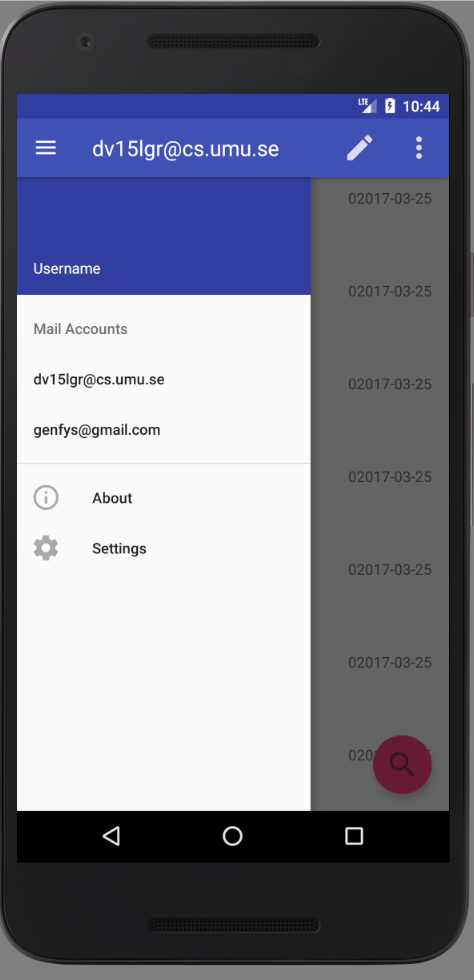
\includegraphics[width=0.5\textwidth]{nav_drawer}
    \caption{\textit{The main view of Apple Mail has three columns: `Mailbox List',
    `Mail List' and `Mail Details'. The `Mailbox List' column is however
    hidden in the standard configuration.}}
\end{figure}

The Navigation drawer offers secondary functionality which relates mostly to
mailbox administration and organisation, correspondigly to the `Mailbox List'
slider column in `Apple Mail'  By default, the inboxes of
all configured mail accounts is merged into the `Mail Message List' view. In the
the navigation drawer, single accounts can be chosen by tapping on them. This
short tap will close the navigation drawer and with a short delay visibly switch
the content of the `Mail Message List' to make the user aware of the selection
he made. A long press on the mail account will open a configuration dialog.

Below the mail accounts, there is a further menu item to access general app
settings.

\subsubsection{Mail Message Viewer}
The `Mail Message View' is opened by tapping on a individual `Mail Message' in
the `Mail Message List' view. As outlined in figure
\ref{fig:hand_design}(rightmost drawing), this view will be composed by an
`ExpandableListView' to structure the history of an mail conversation. The most
recent mail message will be in expanded form, showing the actual message. All
prior messages in a ongoing conversation will be collapsed. The toolbar here
contains a navigation icon on the left edge to go back to the `Mail Message
List'. On the right side of the toolbar is one `ImageButton' for replying the
message and one with the `vertical overflow menu' icon which will open a menu
for secondary functionality.

The reply button will by default start the `Mail Message Editor' Fragment in
`reply-to-sender' mode. A long press on the reply button will open a menu that
provides the `Reply-All' and `Forward' functionality.


\subsubsection{Mail Message Editor}
The `Mail Message Editor' is implemented as a Fragment. The view has a usual
toolbar that with a back navigation on the left edge. In the middle, the message
mode (`Reply', `Reply-All', `Forward') is indicated. At the right edge a `Send
Message' and a `vertical overflow menu' ImageButton is placed. The latter hosts
manual `Message Attachment' functionality which is considered to be of lower importance
in a mobile app. Therefore this functionality is only accessible through the
`vertical overflow menu'. Usually a user will send an attachement out of the
application that handles the type of attachemnt. Then the mail client can be
started by an implicit intent, automatically attaching the object to be sent.

The rest of the UI is split  into three parts: the  header with send mail
account, recipient and message topic, the message edit text area and a slide-in
keyboard to write the actual message. The address field is automatically set
in the case of `Reply' mode. Tapping in the address field will open a contacts
organizer using an implicit intent.

\section{Adapting the Mobile Mail Client from Android to iOS}
To adapt the described mail client app from Android to iOS, mainly two documents
were consulted as guidelines: The general `Human Interface Guidelines' from
Apple (\cite{apple_ios_design}) and a chapter about platform adaption in the
Google Material Design Guidelines (\cite{adapt_ios}).

One change in the general structure of the app is related to the different
interpretation of gestures between Android and iOS: Left to right edge swipe
on iOS is to go back one screen while in Android, when available, it will open
the navigation drawer as described earlier. Hence, instead of a navigation drawer
to choose the current mail account, a speparate screen has to be implemented
on iOS \cite{adapt_ios}.

Besides this, there are a number of obvious details such as switching the font
from `Roboto' on Android to `San Francisco' on iOS. It as further assumed that
for control elements such as switches and checkboxes the corresponding native
versions on iOS are used.





\addcontentsline{toc}{section}{\refname}
\bibliography{references}

\end{document}
